\noindent

\includegraphics[height=1.25cm]{images/pictograms/replication}

\includegraphics[height=1.25cm]{images/pictograms/benchmark}

\includegraphics[height=1.25cm]{images/pictograms/under_construction}

\includegraphics[height=1.25cm]{images/pictograms/pic}

\includegraphics[height=1.25cm]{images/pictograms/nonlinear}

\includegraphics[height=1.25cm]{images/pictograms/paraview}

\includegraphics[height=1.25cm]{images/pictograms/publication}
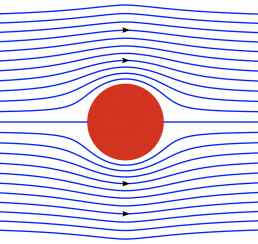
\includegraphics[height=1.25cm]{images/pictograms/streamfunction}


%%%%%%%%%%%%%%%%%%%%%%%%%%%%%%%%%%%%%%%%%%%%%%%%%%%%%%%%%%%%%%%%%%%%%%%%%%%%%%%%%%%%%%%%%%%%%%%%%%%

\begin{flushright} {\tiny {\color{gray} python\_codes/fieldstone\_156/text.tex}} \end{flushright}

%\lstinputlisting[language=bash,basicstyle=\small]{python_codes/template_keywords.key}

\par\noindent\rule{\textwidth}{0.4pt}

\begin{center}
\inpython
{\small Code: \url{https://github.com/cedrict/fieldstone/tree/master/python_codes/fieldstone_156}}
\end{center}

\par\noindent\rule{\textwidth}{0.4pt}

%%%%%%%%%%%%%%%%%%%%%%%%%%%%%%%%%%%%%%%%%%%%%%%%%%%%%%%%%%%%%%%%%%%%%%%%%%%%%%%%%%%%%%%%%%%%%%%%%%%

This \stone is inspired by and is meant to be an incomplete 
replication of \textcite{ketu90} (1990). Most of the text
below is copied verbatim from the paper (but not the codes nor the results).
Note that the same equations can be found in \textcite{kell93} (1993).
It turns out that the Lorenz equations are actually a staple of chaos theory and there 
is {\it a lot} of literature about these\footnote{\url{https://en.wikipedia.org/wiki/Lorenz_system}}.
Of relevance is the paper: \textcite{sttu89} (1989).

The major goals of this work are to generate a flow in two
dimensions that is chaotic in both space and time and
to calculate the deformation of a strain marker in that flow.
The flow is confined to a box of length $w$ and detph $h$.
The stream function is specified as follows:
\begin{equation}
\Psi = 
\left(
\frac{\lambda \sqrt 2}{\pi^2}
\right)
\sin \pi y'
\left\{
B(t') \sin \frac{\pi x'}{\lambda}
+[C(t')-27]\sin \frac{2 \pi x'}{\lambda}
\right\}
\label{eq:ketupsi}
\end{equation}
where $x'=x/h$, $y'=y/h$, $\lambda=w/h$ and $t'$ is the nondimensional
time. 
$B$ and $C$ are time-dependent driver of the flow. This solution satisfies 
conservation of mass and free slip conditions. 
The flow contains either one or two convection cells within the box,
depending on the magnitude of $B$ and $C$.
As $B$ and $C$ vary smoothly but chaotically in time, the flow will oscillate
smoothly but chaotically between one and two cells. 

The flow is driven using the solutions to the Lorenz equations in the chaotic regime:
\begin{eqnarray}
\frac{\partial A}{\partial t'} &=& -\sigma A + \sigma B \label{eq:Lorenz1}\\ 
\frac{\partial B}{\partial t'} &=& -AC + rA -B \label{eq:Lorenz2}\\ 
\frac{\partial C}{\partial t'} &=& AB - bC \label{eq:Lorenz3}
\end{eqnarray}
where $\sigma$, $r$, and $b$ are parameters and $t'=\pi^2 (1+\lambda^{-2}) \kappa t /h^2$
is the nondimensional time with $b=4/(1+\lambda^{-2})$ and $\kappa$ the thermal diffusivity. 

These are numerically integrated to find the time dependence of the solution. 
The parameters $\sigma$ and $r$ represent the Prandtl number  and the ratio
of the Rayleigh number to the critical Rayleigh number for the onset of convection.

In the study the authors use: $r=28$, $\sigma=10$, and $b=8/3$ ($\lambda=\sqrt 2$ since
$w=\sqrt{2}$ and $h=1$).
The solution to this problem has three fixed points, corresponding to
steady flows:

\begin{itemize}
\item $A=B=C=0$ which corresponds to no convection;
\item $A=B=6\sqrt 2$ and $C=27$;
\item $A=B=-6\sqrt 2$ and $C=27$.
\end{itemize}
These steady solutions are unstable, however, and after an initial transient, the solutions 
to the equations above approach the strange 
attractor\footnote{\url{https://en.wikipedia.org/wiki/Attractor}} in $A-B-C$ space.
The solution spirals around the fixed points $A=B=6\sqrt 2$, $C=27$ and 
$A=B=-6\sqrt 2$, $C=27$. It is however non repeating, and the solution is highly sensitive to the initial 
conditions. 

In the physical $x-y$ space, the flow obtained from Lorenz's
model is chaotic in time but not space; a particle follows
a closed path, corresponding to a single streamline, but
its position on that path and its velocity are chaotic in time.
This is unlikely to occur in real fluids, and the Lorenz model 
has very limited direct applicability to real thermal flows.

Also, the Lorenz model cannot be directly applied to mantle convection, 
because at infinite Prandtl number, the chaotic behavior disappears and the Lorenz 
model reverts to steady convection.

The velocity field is obtained as follows\footnote{The authors use a different 
convention for the minus sign so these velocities are opposites of those in the paper.}:
\begin{eqnarray}
u'(x',y') 
&=& \frac{\partial \Psi}{\partial y'} 
= \left(
\frac{\lambda \sqrt 2}{\pi}
\right)
\cos \pi y'
\left\{
B(t') \sin \frac{\pi x'}{\lambda}
+[C(t')-27]\sin \frac{2 \pi x'}{\lambda}
\right\} \nn\\
v'(x',y') 
&=& -\frac{\partial \Psi}{\partial x'} 
=-
\left(
\frac{ \sqrt 2}{\pi}
\right)
\sin \pi y'
\left\{
B(t') \cos \frac{\pi x'}{\lambda}
+2[C(t')-27]\cos \frac{2 \pi x'}{\lambda}
\right\}
\end{eqnarray}
We can easily verify that $u'(x'=0)=u'(x'=w)=0$ and
$v'(x',y'=0)=v'(x',y'=1)=0$.

The evolution of the flow is shown in the figure here under, 
which contains a projection of the solution of the Lorenz equations 
onto the $B-C$ plane:

\begin{center}
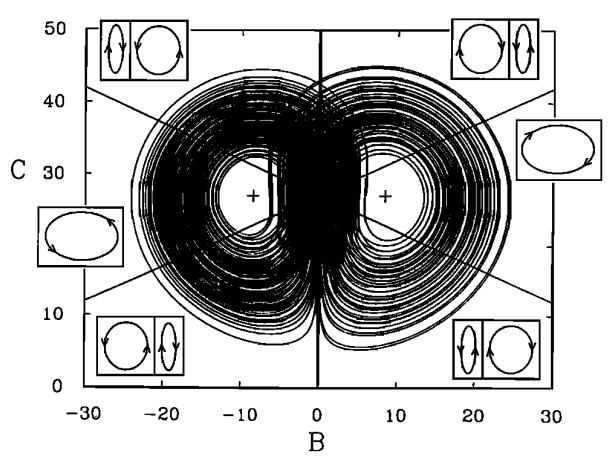
\includegraphics[width=10cm]{python_codes/fieldstone_156/images/ketu90a}\\
{\captionfont Evolution of the Lorenz variables $B$ and $C$,
which govern the time-dependent flow of equation \eqref{eq:ketupsi}.
This is the solution to the Lorenz equations
\eqref{eq:Lorenz1}-\eqref{eq:Lorenz3} projected onto the $B-C$ plane. It is calculated
using  $\sigma$=10, $r$=28, and $b = 8/3$. The inset figures are
schematics of the streamlines of Eq.~\eqref{eq:ketupsi} corresponding
different values of $B$ and $C$. The flow used in the mixing 
calculations oscillates smoothly between one and two cells.}
\end{center}

The figure is divided into regions corresponding
to the differing flow regimes. The inset figures
show schematically the streamlines obtained for
different values of $B$ and $C$. Though the streamlines
are closed at all times, particle trajectories are not, and
the resulting flow has space-filling particle paths.

A representative particle path is shown in the next figure
after times of $t'=1$ (one overturn time), $t'=10$, and $t'=100$.
The flow is space-filling in that a particle will eventually
migrate to every point in the box. 


\begin{center}
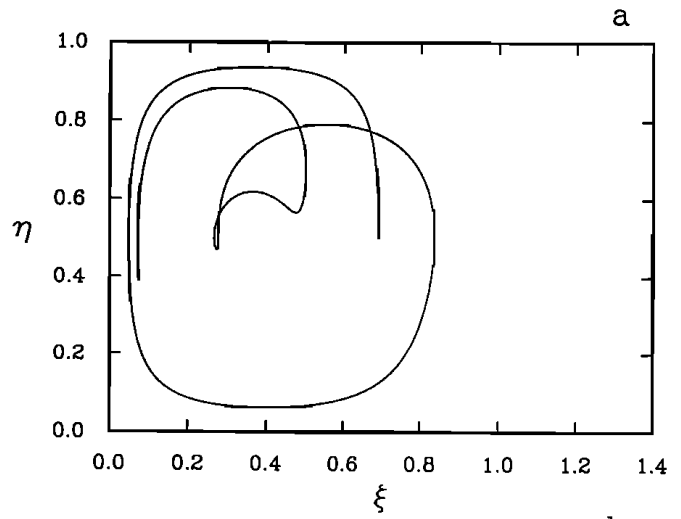
\includegraphics[width=5.7cm]{python_codes/fieldstone_156/images/ketu90b}
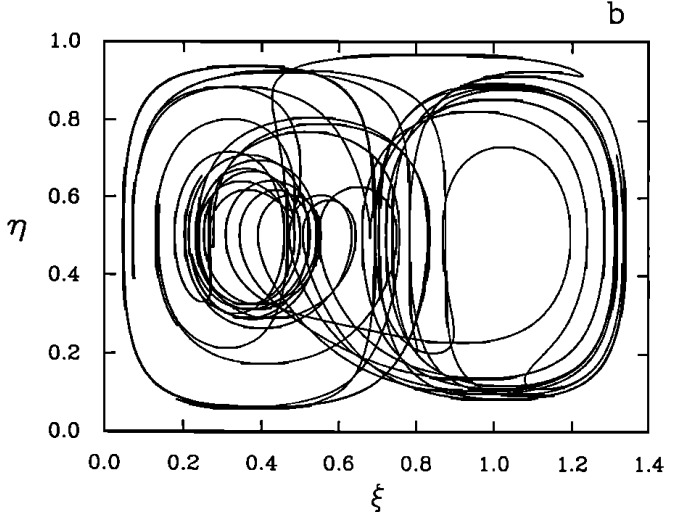
\includegraphics[width=5.7cm]{python_codes/fieldstone_156/images/ketu90c}
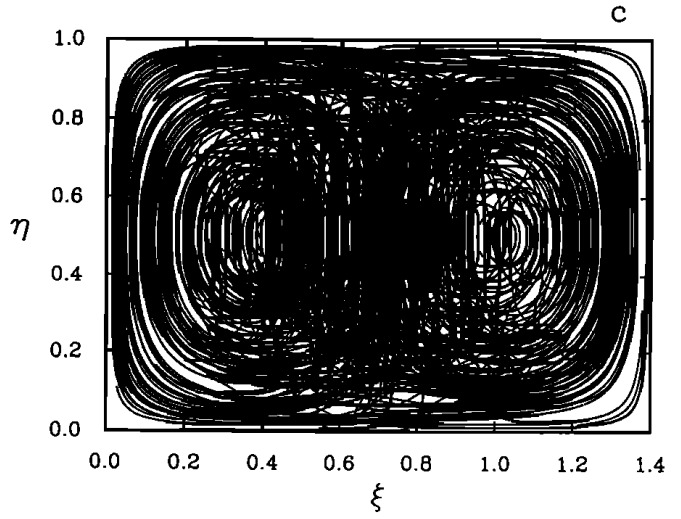
\includegraphics[width=5.7cm]{python_codes/fieldstone_156/images/ketu90d}\\
{\captionfont 
Particle trajectory in the chaotic flow. The particle 
path is shown after times of (a) $t'=1$, (b) $t'=10$, 
and (c) $t'=100$. The particle is initially positioned
at the center of the box.
}
\end{center}


A group of particles
which are initially clustered close together will eventually 
be driven apart and scattered evenly throughout the box:

\begin{center}
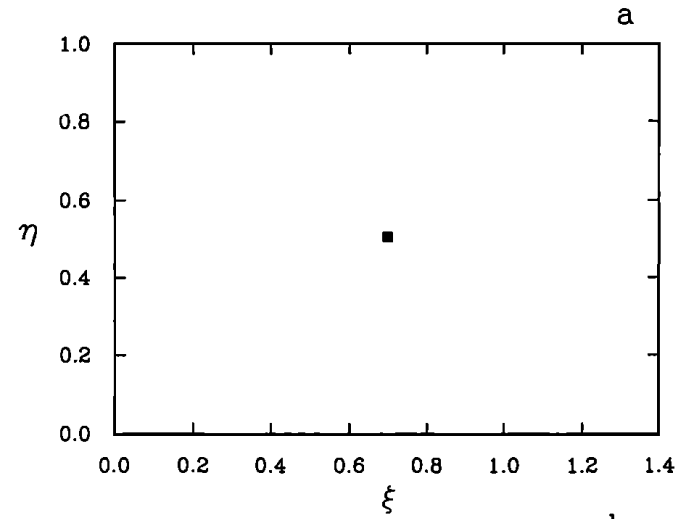
\includegraphics[width=5.7cm]{python_codes/fieldstone_156/images/ketu90e}
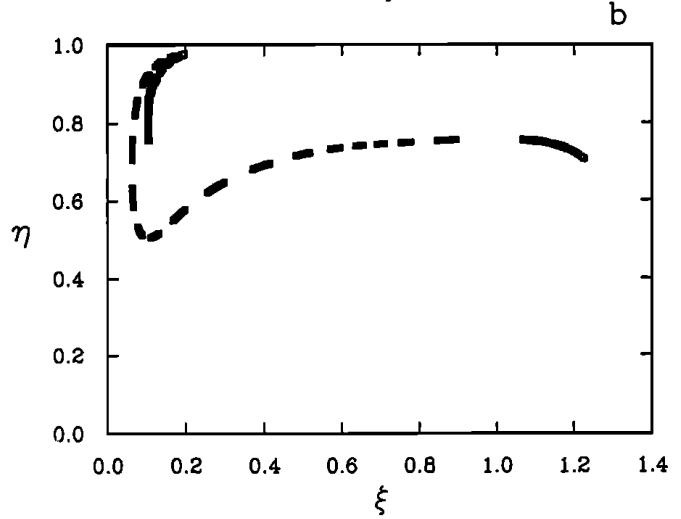
\includegraphics[width=5.7cm]{python_codes/fieldstone_156/images/ketu90f}
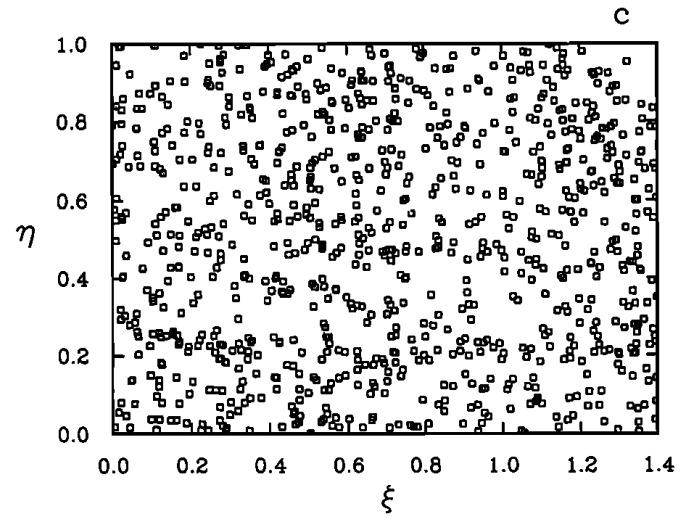
\includegraphics[width=5.7cm]{python_codes/fieldstone_156/images/ketu90g}\\
{
Scattering of a cluster of particles in the chaotic flow.
(a) 900 particles are placed near the center of the box, 
and their positions are tracked and plotted after times 
of (b) $t'=1$ and (c) $t'=10$.
}
\end{center}

%%%%%%%%%%%%%%%%%%%%%%%%%%%%%%%%%%%%%%%%%%%%%%%%%%%%%%%%%%%%%%%%%
\subsection*{What we find online}

%............................
\subsubsection*{Approach 1}

There is a Wikipedia entry\footnote{\url{https://en.wikipedia.org/wiki/Lorenz_system}} 
for the Lorenz system.
As it turns out, it is also run with $s=10$, $\beta=8/3$ and $\rho=28$.
There are also a few codes available, in Matlab, Python and Julia on the page. 
The python one is saved in the folder {\tt wiki} in this \stone. 
It unfortunately implements a first order time integrator so that it will
not be of much use when it comes to accuracy of the results
(I have then also modified the starting point to match mine, i.e. 0,0.5.25).

\begin{center}
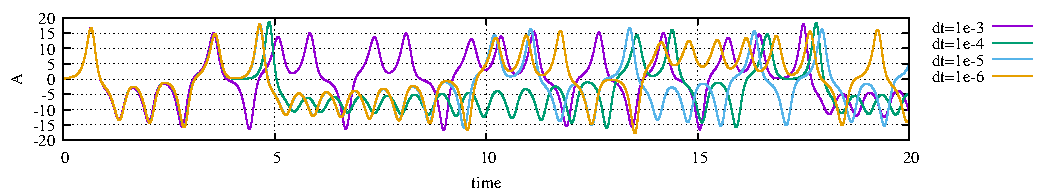
\includegraphics[width=16cm]{python_codes/fieldstone_156/wiki/A.pdf}\\
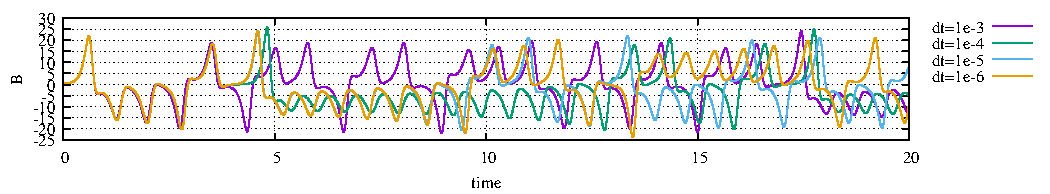
\includegraphics[width=16cm]{python_codes/fieldstone_156/wiki/B.pdf}\\
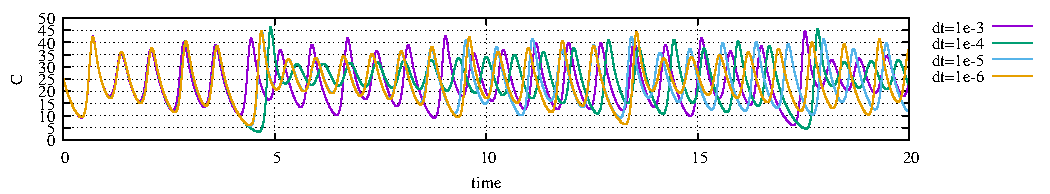
\includegraphics[width=16cm]{python_codes/fieldstone_156/wiki/C.pdf}\\
{\captionfont Given the simplistic integration scheme, we find that 
results diverge after $t'>5$.}\\
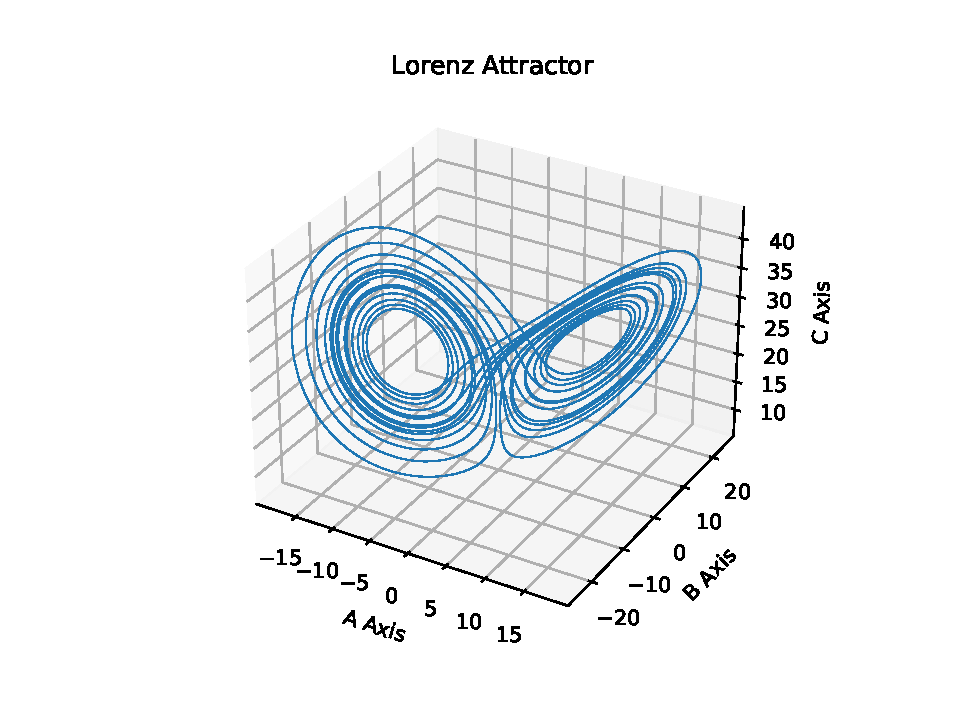
\includegraphics[width=11cm]{python_codes/fieldstone_156/wiki/ABC.pdf}
\end{center}

%............................
\subsubsection*{Approach 2}

I found another similar code\footnote{\url{https://marksmath.org/classes/Fall2020DiffEq/demos/Lorenz.html}}, 
but it now makes use of 'odeint' which seems to be 
deprecated\footnote{\url{https://docs.scipy.org/doc/scipy/reference/generated/scipy.integrate.odeint.html}}.
I am not sure what the method behind odeint actually is.
The code is to be found in the {\tt marksmath} folder. The timestep is set by the user.

\begin{center}
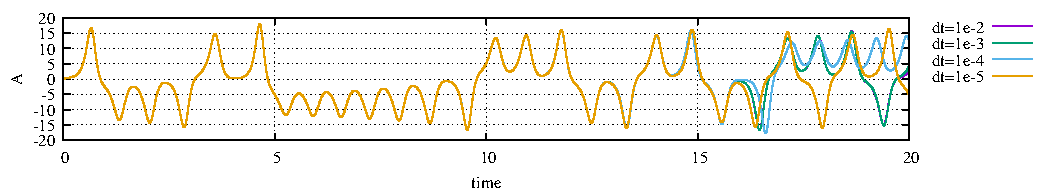
\includegraphics[width=16cm]{python_codes/fieldstone_156/marksmath/A.pdf}\\
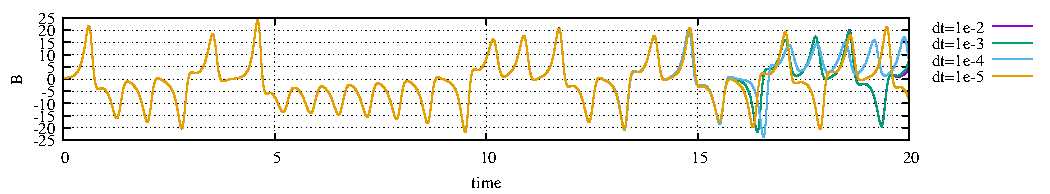
\includegraphics[width=16cm]{python_codes/fieldstone_156/marksmath/B.pdf}\\
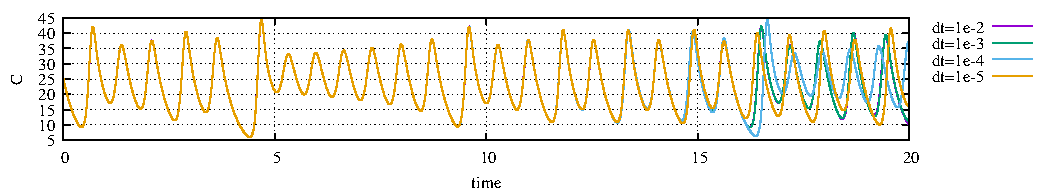
\includegraphics[width=16cm]{python_codes/fieldstone_156/marksmath/C.pdf}\\
{\captionfont Results are much better and only diverge for $t'>15$.}
\end{center}

%............................
\subsubsection*{Approach 3}

We find elsewhere\footnote{\url{https://scipython.com/blog/the-lorenz-attractor/}} 
an even more advanced take on this problem.
It uses the {\python solve\_ivp} 
function\footnote{\url{https://docs.scipy.org/doc/scipy/reference/generated/scipy.integrate.solve_ivp.html}}.
It uses by default RK45, but can be called with RK23, DOP853 (Dormand \& Prince, see hereafter), 
Radau\footnote{\url{https://en.wikipedia.org/wiki/List_of_Runge-Kutta_methods}} and BDF (the last two are implicit 
methods).
The Lorenz function is defined as follows:
\begin{lstlisting}
def lorenz(t, X, sigma, beta, rho):
    u, v, w = X
    up = -sigma*(u - v)
    vp = rho*u - v - u*w
    wp = -beta*w + u*v
    return up, vp, wp
\end{lstlisting}
and a call to {\python solve\_ivp} goes as follows:
\begin{lstlisting}
soln = solve_ivp(lorenz, (0,tmax), (u0,v0,w0), args=(sigma, beta, rho),
                 method='RK23', max_step=maxdt)
\end{lstlisting}

For now the step size is not bounded ({\python maxdt} is infinite)
and determined solely by the integration scheme.

\begin{center}
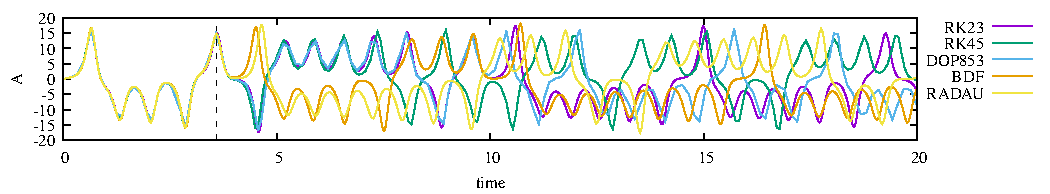
\includegraphics[width=16cm]{python_codes/fieldstone_156/blog/A_auto.pdf}\\
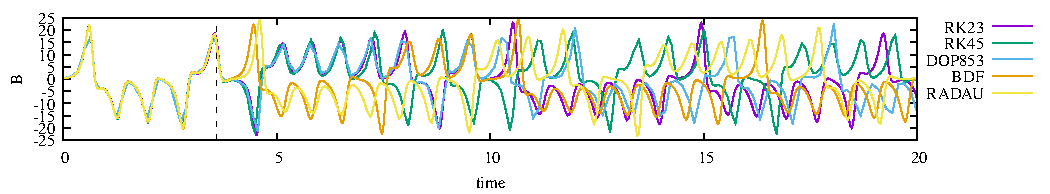
\includegraphics[width=16cm]{python_codes/fieldstone_156/blog/B_auto.pdf}\\
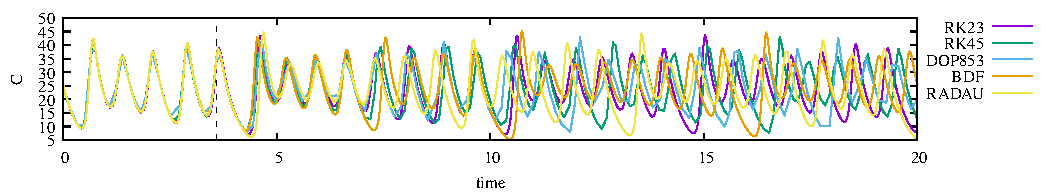
\includegraphics[width=16cm]{python_codes/fieldstone_156/blog/C_auto.pdf}\\
{\captionfont Looking at $A(t')$, we find that at $t'\simeq 4$ the RK-like
methods 'go up' while the Radau \& BDF methods go down. This is raher 
disappointing.}
\end{center}

Looking closer I found out that the total number of time steps used to reach $t'=20$
for each method varies quite a lot:
\begin{center}
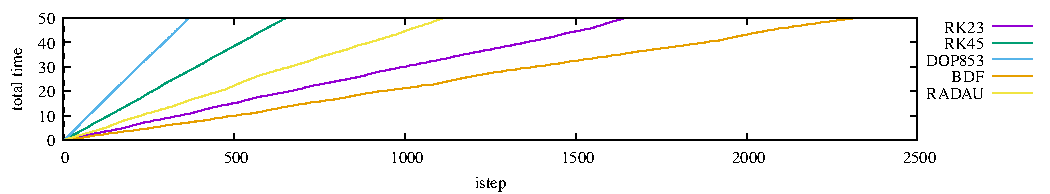
\includegraphics[width=16cm]{python_codes/fieldstone_156/blog/time_auto.pdf}\\
{\captionfont RK23: 1647 steps; RK45: 652 steps $\delta t \simeq 0.077$; DOP853: 369 steps;
Radau: 1114 steps; BDF: 2323 $\delta t \simeq 0.0215$.}  
\end{center}

I feel that we need to try these methods again with much smaller time step.
I therefore set $\delta t=10^{-4}$ for all five methods:

\begin{center}
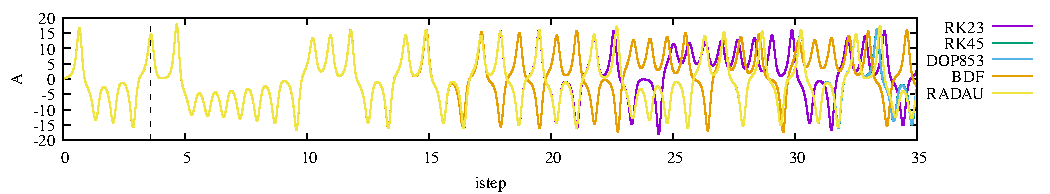
\includegraphics[width=16cm]{python_codes/fieldstone_156/blog/A4.pdf}\\
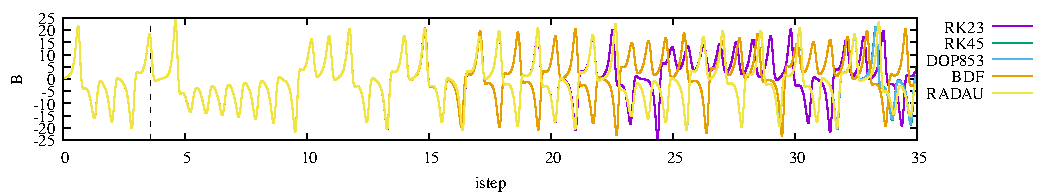
\includegraphics[width=16cm]{python_codes/fieldstone_156/blog/B4.pdf}\\
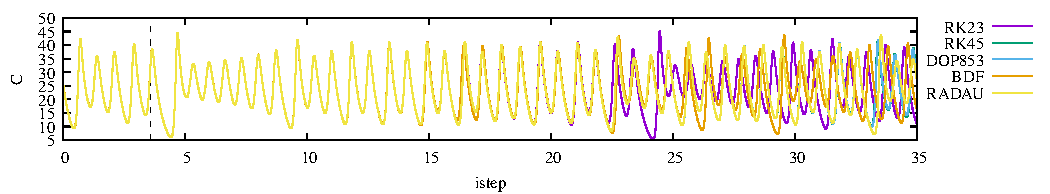
\includegraphics[width=16cm]{python_codes/fieldstone_156/blog/C4.pdf}\\
{\captionfont My hunch was correct and a smaller time step allows 
all the methods to agree up to $t'\simeq 15$.
RK23 unsurprinsigly does not perform as well as the others.}
\end{center}

This is very encouraging so I now set $\delta t=10^{-5}$ for all five methods:

\begin{center}
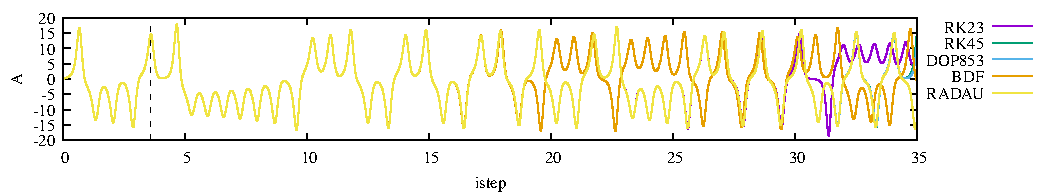
\includegraphics[width=16cm]{python_codes/fieldstone_156/blog/A5.pdf}\\
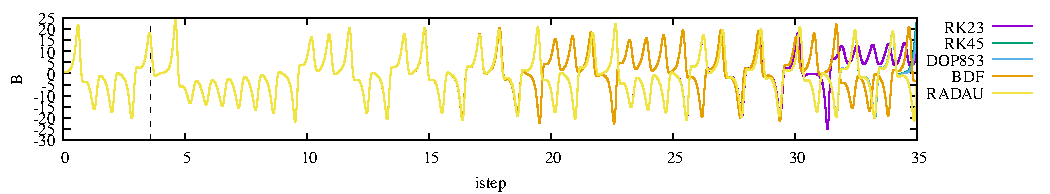
\includegraphics[width=16cm]{python_codes/fieldstone_156/blog/B5.pdf}\\
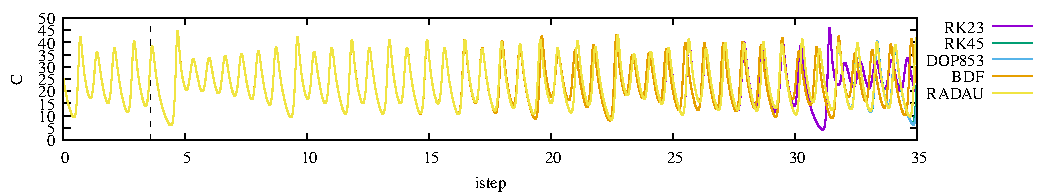
\includegraphics[width=16cm]{python_codes/fieldstone_156/blog/C5.pdf}\\
{\captionfont Surprisingly BDF refuses to yield the same results as all 
other methods.}
\end{center}
In the end, no matter what I try, I cannot seem to get all methods to agree past $t'=30$! 

Let us now try to solve these equations ourselves...

%%%%%%%%%%%%%%%%%%%%%%%%%%%%%%%%%%%%%%%%%%%%%%%%%%%%%%%%%%%%%%%%%
\subsection*{About the code}

The domain is a rectangle of size $L_x,L_y$ with $L_x=w=\sqrt 2$ and $L_y=h=1$
so that $\lambda=w/h=\sqrt 2$ as in the publication (see figures above).
We set $\sigma=10$, $r=28$ and $b=8/3$. 
What we ultimately miss are the initial values for $A,B,C$. We cannot start
with all three equal to zero, otherwise we obtain the solution $A=B=C=0$ solution.
Looking at the first figure in $B-C$ space we see that the values are constrained in 
$[-30,30]\times[0,50]$ so we can set $B=0.5$ and $C=25$ at $t'=0$. 
For now we also set $A=0$ at startup. 

At the moment markers are set on a $40\times 40$ grid in a square 
of size $0.025\times 0.025$ placed in the middle of the domain, and 
they are advected by means of a simple Euler step\footnote{This should be 
improved!}. 

The code then solve Eqs.~\eqref{eq:Lorenz1},\eqref{eq:Lorenz2},\eqref{eq:Lorenz3}.
These are coupled first-order nonlinear equations. From our experience with 
codes found online, this is no good news and 
specific numerical techniques should be used in this case. 

%..........................
\subsubsection*{scheme 1}

To get things started I nevertheless opt for a simplistic approach. 
The time derivatives are discretised by means of 1st order explicit formulas ({\tt scheme 1}):
\begin{eqnarray}
\frac{A^{n+1}-A^n}{\delta t} &=& -\sigma A^n + \sigma B^n \nn\\
\frac{B^{n+1}-B^n}{\delta t} &=& -A^n C^n + rA^n -B^n  \nn\\
\frac{C^{n+1}-C^n}{\delta t} &=& A^n B^n - bC^n \nn
\end{eqnarray}
where the upperscript denotes the timestep. We will use tiny time steps and hope for the best.

Every time that new $B$ and $C$ values are obtained we can use these to compute the 
velocity field and to drive the flow.

\begin{center}
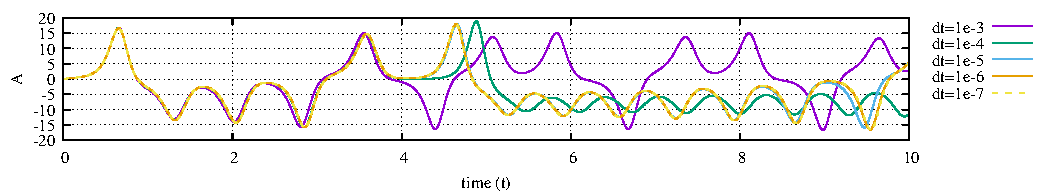
\includegraphics[width=16cm]{python_codes/fieldstone_156/results/scheme1/A.pdf}\\
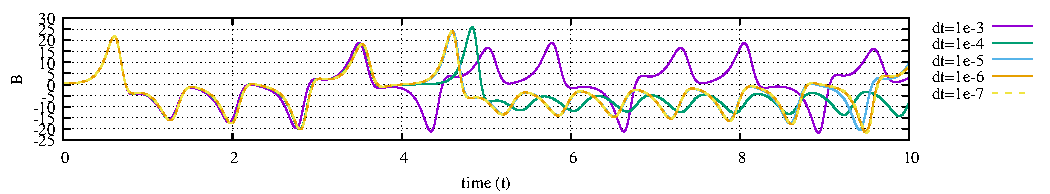
\includegraphics[width=16cm]{python_codes/fieldstone_156/results/scheme1/B.pdf}\\
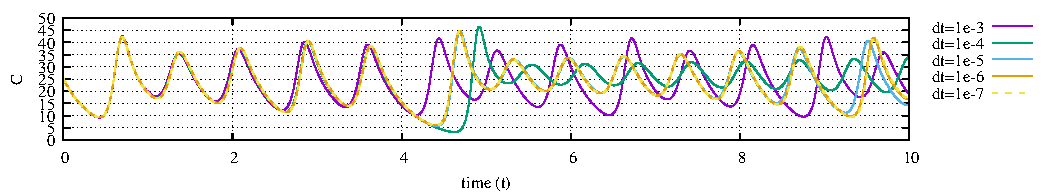
\includegraphics[width=16cm]{python_codes/fieldstone_156/results/scheme1/C.pdf}\\
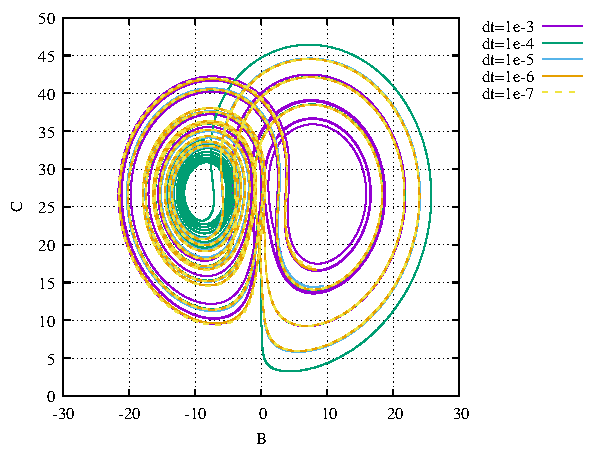
\includegraphics[width=9cm]{python_codes/fieldstone_156/results/scheme1/BC.pdf}\\
{\captionfont Clearly $\delta t=1e-3$ is too large, 
and given the simplistic integration scheme, we find that 
even using very small time steps results diverge after $t'=10$.}
\end{center}


%..........................
\subsubsection*{scheme 2}

Based on these encouraging results, it is now time to look at a more appropriate
scheme to solve the equations.
We can try something very simple, i.e. use updated values of $B$ and $C$ when possible ({\tt scheme 2}):
\begin{eqnarray}
\frac{A^{n+1}-A^n}{\delta t} &=& -\sigma A^n + \sigma B^n \nn\\
\frac{B^{n+1}-B^n}{\delta t} &=& -A^{n+1} C^n + rA^{n+1} -B^n  \nn\\
\frac{C^{n+1}-C^n}{\delta t} &=& A^{n+1} B^{n+1} - bC^n \nn
\end{eqnarray}
i.e.
\begin{eqnarray}
A^{n+1} &=& (-\sigma A^n + \sigma B^n) \delta t + A^n \nn\\
B^{n+1} &=& (-A^{n+1} C^n + rA^{n+1} -B^n ) \delta t+ B^n \nn\\
C^{n+1} &=& (A^{n+1} B^{n+1} - bC^n ) \delta t + C^n \nn
\end{eqnarray}

\begin{center}
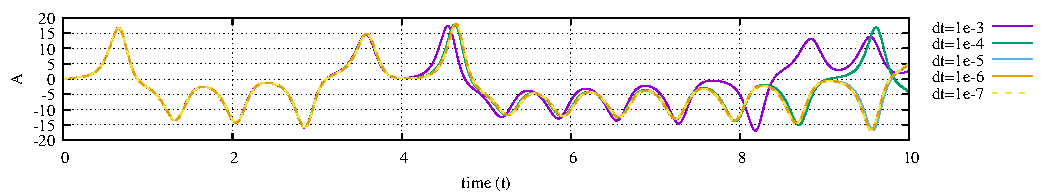
\includegraphics[width=16cm]{python_codes/fieldstone_156/results/scheme2/A.pdf}
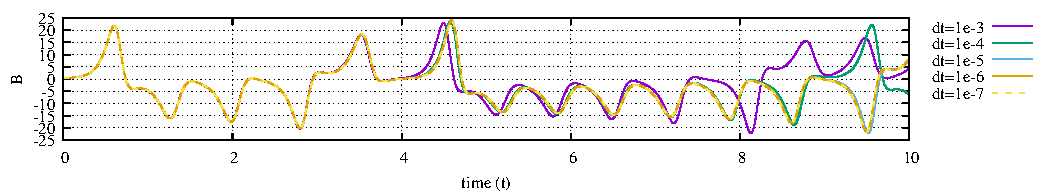
\includegraphics[width=16cm]{python_codes/fieldstone_156/results/scheme2/B.pdf}
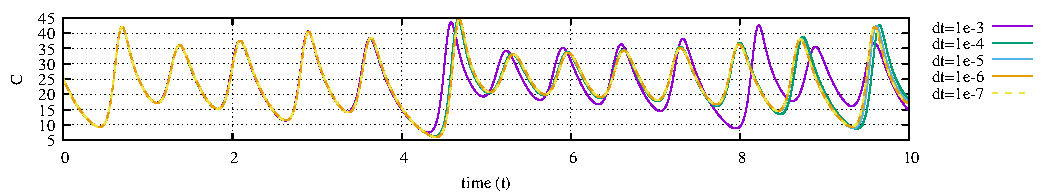
\includegraphics[width=16cm]{python_codes/fieldstone_156/results/scheme2/C.pdf}\\
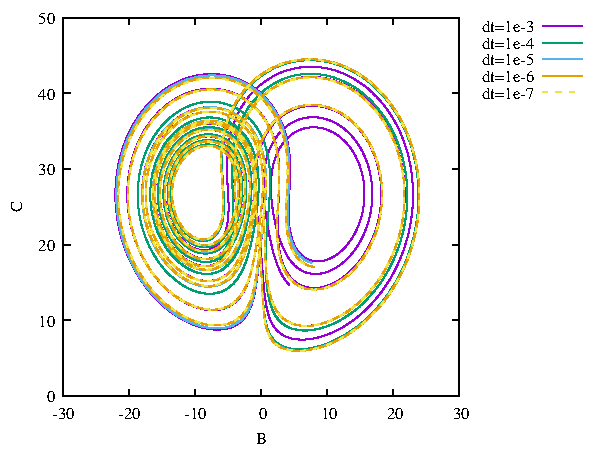
\includegraphics[width=9cm]{python_codes/fieldstone_156/results/scheme2/BC.pdf}\\
\end{center}

This is somewhat better, lines with 'large' $\delta t$ are closer to the reference
$\delta t=5\cdot 10^{-5}$ line. 
I have also made a nice video of what happens:
\url{https://www.youtube.com/watch?v=Bd9rRSSbH1o}.

\begin{center}
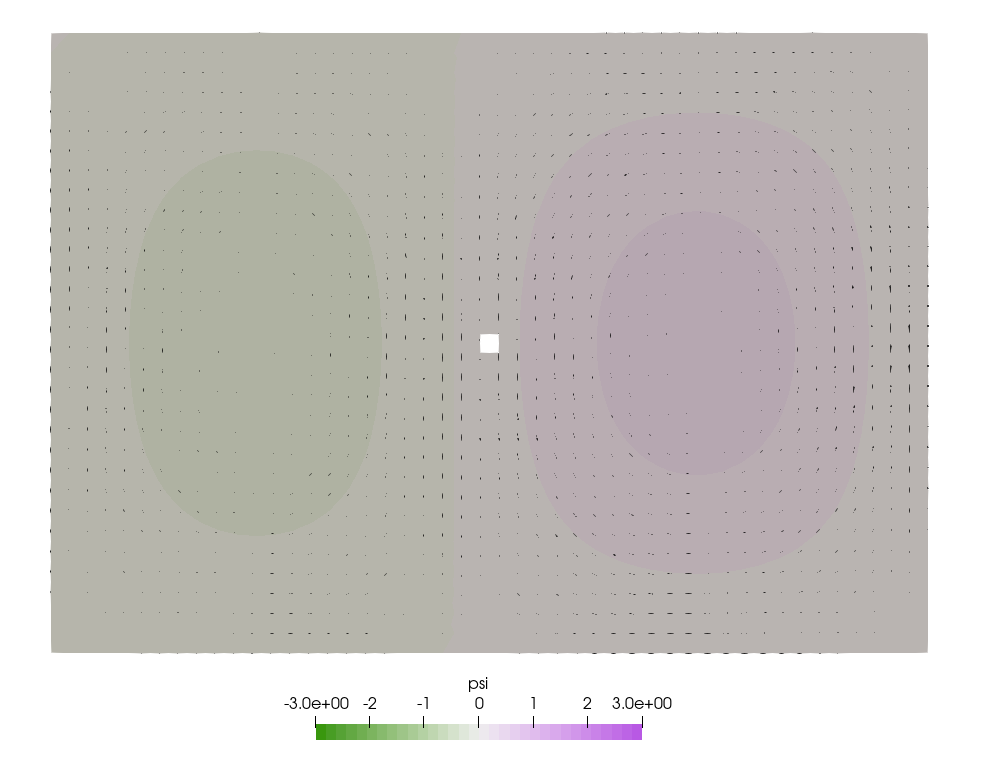
\includegraphics[width=8cm]{python_codes/fieldstone_156/results/scheme2/psi0000}
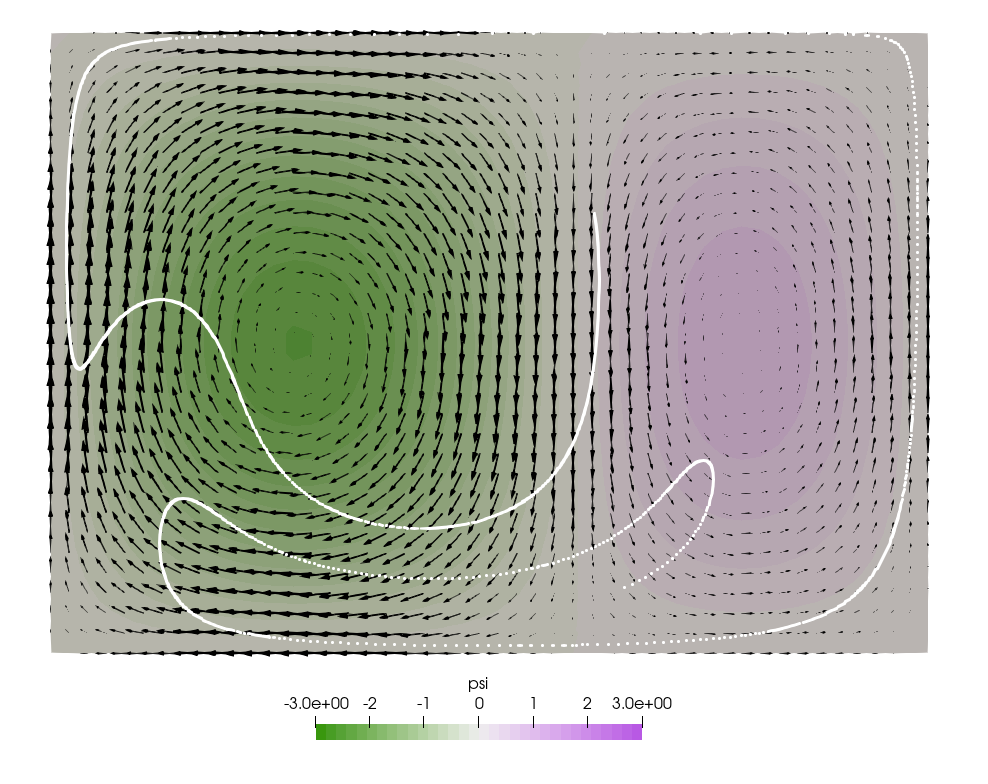
\includegraphics[width=8cm]{python_codes/fieldstone_156/results/scheme2/psi0100}\\
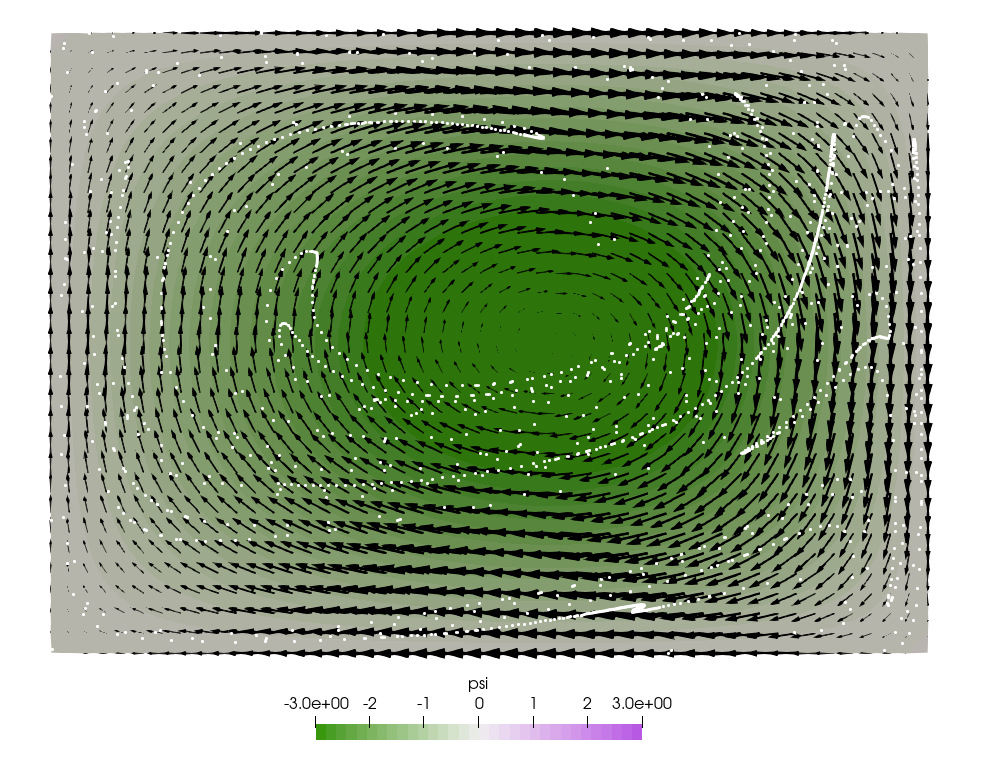
\includegraphics[width=8cm]{python_codes/fieldstone_156/results/scheme2/psi0200}
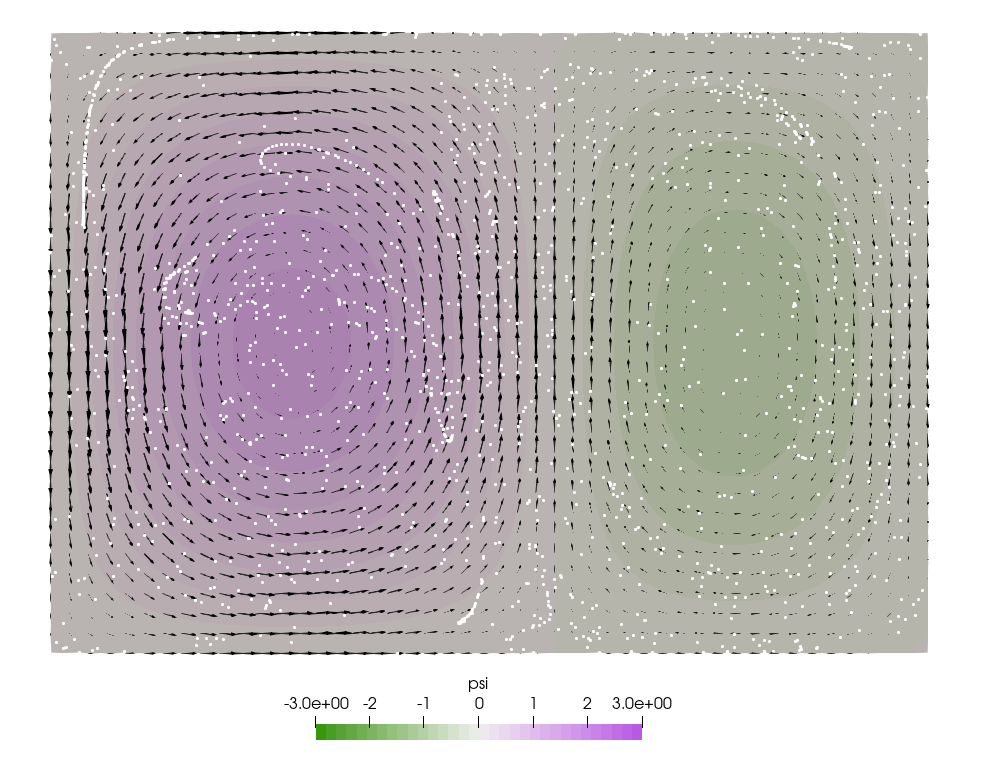
\includegraphics[width=8cm]{python_codes/fieldstone_156/results/scheme2/psi0300}\\
{\captionfont Markers, stream function field and velocity arrows. Obtained with $\delta t=10^{-4}$.}
\end{center}


%..........................
\subsubsection*{scheme 3}

{\tt scheme=3} does a few (fixed point) iterations at each time step:

\begin{center}
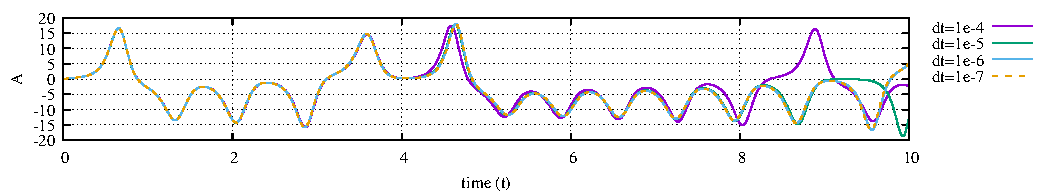
\includegraphics[width=16cm]{python_codes/fieldstone_156/results/scheme3/A.pdf}
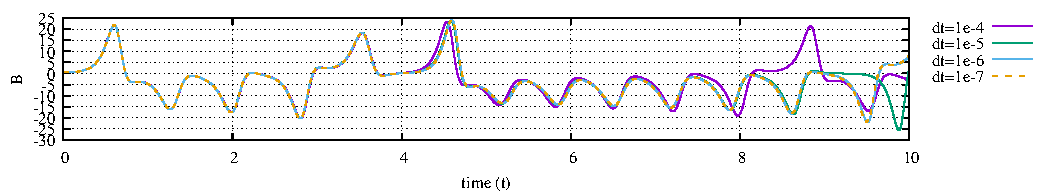
\includegraphics[width=16cm]{python_codes/fieldstone_156/results/scheme3/B.pdf}
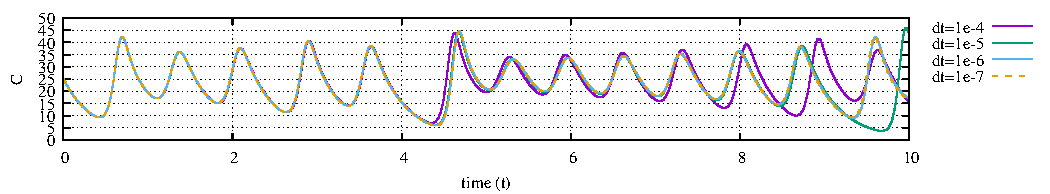
\includegraphics[width=16cm]{python_codes/fieldstone_156/results/scheme3/C.pdf}\\
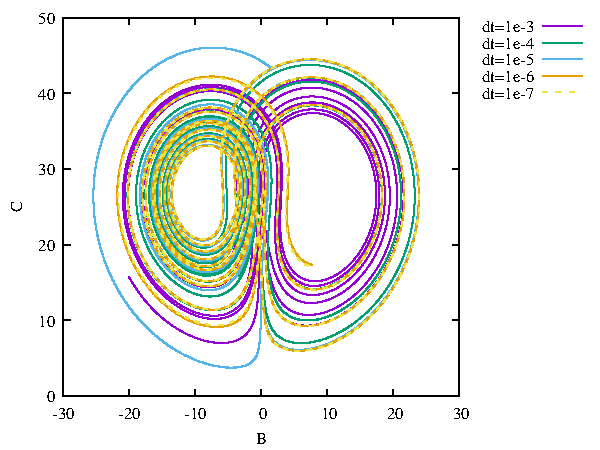
\includegraphics[width=9cm]{python_codes/fieldstone_156/results/scheme3/BC.pdf}\\
{\captionfont Not sure what to make of it... looks different than the other two...}
\end{center}

%...........................
\subsubsection*{Comparing results from schemes 1, 2 and 3}

We can compare the three schemes (1,2,3) when the smallest time 
step $\delta t=10^{-7}$ is used.
We find that up to $t'=10$ they agree very well.
\begin{center}
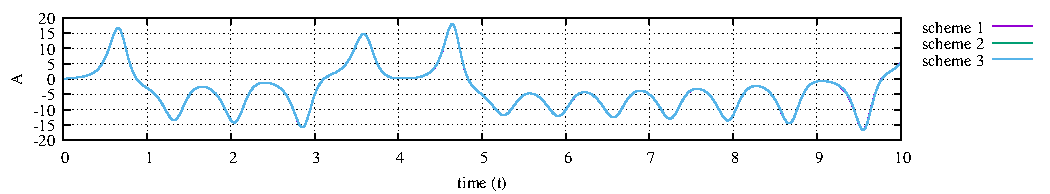
\includegraphics[width=16cm]{python_codes/fieldstone_156/results/A.pdf}\\
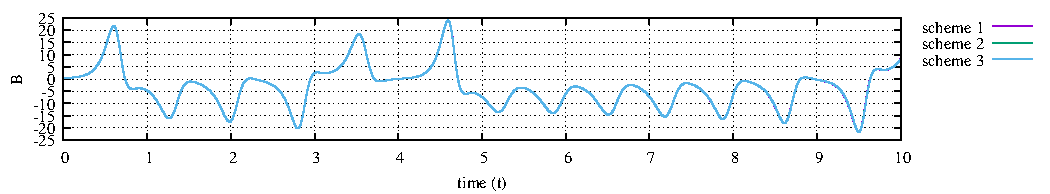
\includegraphics[width=16cm]{python_codes/fieldstone_156/results/B.pdf}\\
\includegraphics[width=16cm]{python_codes/fieldstone_156/results/C.pdf}
\end{center}


%...........................
\subsubsection*{scheme 4}

Let us now switch to the standard 4th order 
Runge-Kutta method\footnote{\url{https://en.wikipedia.org/wiki/Runge-Kutta_methods}},
that we denote by {\tt scheme=4}. It is often described as follows.
Let an initial value problem be specified as follows:
\[
dy/dt = f (t,y) , y(t_0) = y_0
\]
Here $y$ is an unknown function (scalar or vector) of time $t$, 
which we would like to approximate; we are told that $dy/dt$, 
the rate at which $y$ changes, is a function of $t$ 
and of $y$ itself. At the initial time $t_0$ the corresponding $y$ value 
is $y_0$. The function $f$ and the initial conditions $t_0$, $y_0$ are given. 
Now we pick a step-size $h> 0$ and define: 
\[
y_{n+1}= y_n + \frac{h}{6}(k_1+2k_2+2k_3+k_4) 
\qquad
\qquad
\qquad
t_{n+1}=t_n + h
\]
for $n = 0, 1, 2, 3, ...$, using
\begin{eqnarray}
k_1 &=& f(t_n,y_n) \nn\\
k_2 &=& f(t_n+\frac{h}{2},y_n+\frac{h}{2}k_1) \nn\\
k_3 &=& f(t_n+\frac{h}{2},y_n+\frac{h}{2}k_2) \nn\\
k_4 &=& f(t_n+h,y_n+ h k_3) \nn
\end{eqnarray}
In this case, we have
\[
\frac{d}{dt} 
\left(
\begin{array}{c}
A\\B\\C
\end{array}
\right)
=\vec{f}(A,B,C)
\]
This is probably a somewhat naive attempt at using RK4 for coupled PDEs.
Note that Runge-Kutta methods are discussed in Section~\ref{MMM-ss:rkm}.
We find that even when the time step is 'large' the solutions are 
identical to our most accurate solutions so far. 
I therefore increase the final time to $t'=35$.
We find that differences start to show up at the $t'\simeq 22$ mark. 

\begin{center}
\includegraphics[width=16cm]{python_codes/fieldstone_156/results/scheme4/A.pdf}\\
\includegraphics[width=16cm]{python_codes/fieldstone_156/results/scheme4/B.pdf}\\
\includegraphics[width=16cm]{python_codes/fieldstone_156/results/scheme4/C.pdf}\\
\includegraphics[width=9cm]{python_codes/fieldstone_156/results/scheme4/BC.pdf}
\end{center}

This approach is documented in this video \url{https://www.youtube.com/watch?v=EXvLju3DLMY}
or this one \url{https://www.youtube.com/watch?v=5CXhHx56COo}.

%...........................
\subsubsection*{scheme 5}

The Runge-Kutta method of scheme 4 is only one of many, and several other ones which are 
more accurate exist. 
Let us try the so-called 3/8-rule one .

\begin{center}
\includegraphics[width=16cm]{python_codes/fieldstone_156/results/scheme5/A.pdf}\\
\includegraphics[width=16cm]{python_codes/fieldstone_156/results/scheme5/B.pdf}\\
\includegraphics[width=16cm]{python_codes/fieldstone_156/results/scheme5/C.pdf}\\
\includegraphics[width=9cm]{python_codes/fieldstone_156/results/scheme5/BC.pdf}
\end{center}

%...........................
\subsubsection*{scheme 6}

We can also try the Runge-Kutta-Fehlberg Method (RKF45, \cite{dopr80}), which is 
5th order. 
The particularity of this method is that from the same Butcher Tableau one 
can produce a 4th-order approximation $\tilde{A}$ and a 5th-order approximation $A$:
\begin{eqnarray}
\tilde{A}_{n+1}&=&A_n + \frac{25}{216}A_1 + \frac{1408}{2565}A_3+\frac{2197}{4101}A_4 -\frac15 A_5 \nn\\
A_{n+1}&=&A_n + \frac{16}{135}A_1 + \frac{6656}{12825}A_3+\frac{28561}{56430}A_4 \nn
-\frac{9}{50} A_5 + \frac{2}{55} A_6
\end{eqnarray}
I then define 
\begin{eqnarray}
R_A=\frac{1}{\delta t} | \tilde{A}_{n+1} - A_{n+1} | \nn\\
R_B=\frac{1}{\delta t} | \tilde{B}_{n+1} - B_{n+1} | \nn\\
R_C=\frac{1}{\delta t} | \tilde{C}_{n+1} - C_{n+1} | \nn
\end{eqnarray}
and the new time step is $s\cdot \delta t$, with $s=min(s_A,s_B,s_C)$
and\footnote{I have a doubt about the exponent: 1/4 or 1/5?} 
\[
s_A= \left(\frac{tol}{2R_A}\right)^\frac14 \qquad \qquad 
s_B= \left(\frac{tol}{2R_B}\right)^\frac14 \qquad \qquad 
s_C= \left(\frac{tol}{2R_C}\right)^\frac14
\]
This means that in this case we do not control the value of the timestep
directly, but rather indirectly by means of the tolerance value.
We find that for $tol=1e-7,8,9$ we obtain a timestep around $10^{-4}$.
\begin{center}
\includegraphics[width=7cm]{python_codes/fieldstone_156/results/scheme6/dt.pdf}
\includegraphics[width=7cm]{python_codes/fieldstone_156/results/scheme6/sABC.pdf}
\end{center}
and the results are as follows:
\begin{center}
\includegraphics[width=16cm]{python_codes/fieldstone_156/results/scheme6/A.pdf}
\includegraphics[width=16cm]{python_codes/fieldstone_156/results/scheme6/B.pdf}
\includegraphics[width=16cm]{python_codes/fieldstone_156/results/scheme6/C.pdf}
\end{center}


%...........................
\subsubsection*{scheme 7}

I then went `all in' and decided to implement a 9th-order Dormand-Prince (often
called 'ode87'), see Section~\ref{MMM-ss:rkm} or also
\url{https://nl.mathworks.com/matlabcentral/fileexchange/3616-ode87-integrator}.

\begin{center}
\includegraphics[width=16cm]{python_codes/fieldstone_156/results/scheme7/A.pdf}
\includegraphics[width=16cm]{python_codes/fieldstone_156/results/scheme7/B.pdf}
\includegraphics[width=16cm]{python_codes/fieldstone_156/results/scheme7/C.pdf}
\end{center}
I have also tried to set $\delta t$ to small values, instead of the tolerance.
I recovered similar results as when DOP853 was used in Approach 3 (see earlier).

\vspace{1cm}

The conclusion so far is that using (very) high order methods does not 
yield stable results past $t'>30$.
Based on all this I am actually wondering whether it is actually impossible 
to have results overlap past $t'>30$ because of the chaotic nature of the 
equations themselves.


